\documentclass[14pt, a4paper]{report}
\usepackage{mathtext}
\usepackage[T2A]{fontenc}
\usepackage[utf8]{inputenc}
\usepackage[russian]{babel}
\usepackage{multirow}
\usepackage{slashbox}
\usepackage{makecell}
\usepackage{graphicx}
\usepackage{physics}
\usepackage{amstext}
\usepackage{caption}
\usepackage{subcaption}
\usepackage{cmap}
\usepackage{float}
\usepackage{siunitx}

\renewcommand{\thesection}{\arabic{section}.}
\renewcommand{\thesubsection}{\arabic{section}.\arabic{subsection}.}

\title{\textbf{Отчет о выполнении лабораторной работы 4.4.2 "Фазовая дифракционная решётка"}}
\author{Алпатова Александра, Калашников Михаил, Б03-205}
\date{}

\begin{document}
\maketitle

\textbf{Цель работы:}
Знакомство с работой и настройкой гониометра Г5, определение спектральных характеристик фазовой решётки (эшелетта).
\newline

\textbf{В работе используются:}
\begin{itemize}
\item гониометр,
\item эшелетт,
\item ртутная лампа.
\end{itemize}

\section{Теоретические сведения}

\begin{figure}[H]
	\centering
	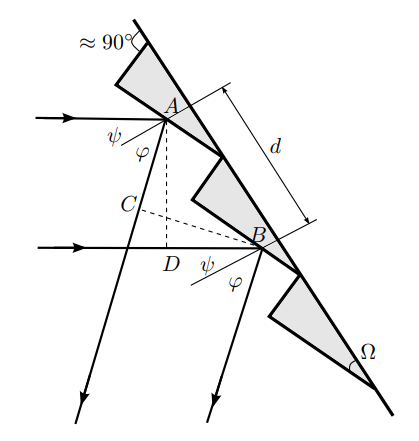
\includegraphics[width=0.5\linewidth]{../images/442_7}
	\caption{Профиль фазовой дифракционной решётки; дифракция световой волны}
	\label{fig:решёткаВпрофиль}
\end{figure}

В современных спектральных приборах широко используются отражательные решётки с треугольным профилем штриха (рис. \ref{fig:решёткаВпрофиль}), они способны концентрировать до $ 70–80\% $ падающего излучения в рабочий порядок спектра. Отражательная решётка, в которой угол $ \Omega $ между рабочей гранью и плоскостью решётки не превышает $ 20^\circ $, называется эшелеттом. Для эшелетта, варьируя угол скоса и шаг решётки, получают рабочий порядок $ m_р \le 10 $.

Найдём разность хода между лучами на рис. \ref{fig:решёткаВпрофиль}. Условие возникновения спектра порядка $ m $:
\begin{equation}\label{eq:spectreM}
	A C - B D = d (\sin \varphi m- \sin \psi) = m \lambda,
\end{equation}
где $ \psi $ -- угол падения от нормали к решётке, $ \varphi $ -- угол дифракции.
Для нулевого порядка $ \varphi_0 = \psi $. В отличие от амплитудной решётки, нулевой порядок не будет самым ярким. Угол $ \varphi_б $ -- угол блеска, соответствующий максимуму интенсивности света, равен углу зеркального отражения падающей волны от одной ступеньки:
\begin{equation*}\label{key}
	\varphi_б = \psi+ 2 \Omega.
\end{equation*}
Для эшелетта рабочим порядком спектра $  m_р$ будет то целое число, которое соответствует минимальной ошибке решения уравнения $d \sin \varphi_m - \sin \psi = 0 $.

Cчитая, что эшелетт работает в автоколлимационном режиме, то есть свет падает перпендикулярно рабочей грани решётки ($ \psi = -\Omega $) и отражается в обратном направлении ($ \varphi = \Omega $), тогда
\begin{equation}\label{om}
	2 d \sin \Omega = m_р \lambda_р.
\end{equation}
В автоколлимационном режиме дифракция на одной ступеньке-зеркальце описывается так же, как и дифракция на отдельной щели амплитудной решётки с максимумом вблизи $ \varphi \approx 0 $. В отличие от амплитудной решётки, нумерацию порядков для амплитудной решётки, следует сместить на величину $ m_р $.

\section{Проведение эксперимента}

\begin{enumerate}

\setcounter{enumi}{0}

\item Проведем юстировку и настройку гониометра в соответствии с техническим описанием. Настроим коллиматор и зрительную трубу. Установим начало отсчета углов.

\item Установим эшелетт на столик рабочей поверхностью к коллиматору.

\item Приступим к изучению спектра ртутной лампы. Для угла падения света на эшелетт $\psi=\ang{30}$ измерим угловые координаты спектральных линий.

\item Для оценки разрешающей способности измерим угловые координаты линий желтого дублета для различных углов падения.

\end{enumerate}

\section{Обработка данных}

\begin{enumerate}

\item Построим график зависимости $\sin\phi_m-\sin\psi$ от длины волны. Проведя через точки прямую с коэффициентом наклона $k$ можно определить шаг решетки по формуле $d=m/k=5.7\ мкм$.

\begin{figure}[H]
\centering
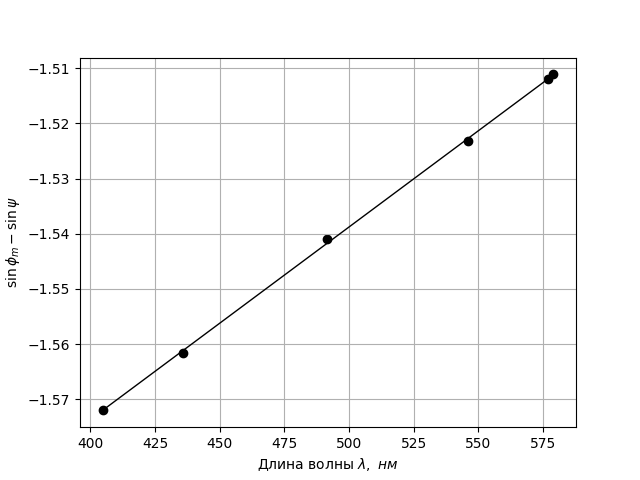
\includegraphics[scale=0.6]{../images/442_1.png}
\caption{График зависимости $\sin\phi_m-\sin\psi$ от длины волны}
\end{figure}

\item Угол скоса рабочей грани эшелетта может быть рассчитан по формуле:
\[\Omega=\arcsin\frac{m_р\lambda_р}{2d}=2.5^\circ\]

\item Рассчитаем экспериментальную угловую дисперсию $D=\frac{\Delta\phi}{\Delta\lambda}$, основываясь на измерениях желтого дублета:

\[D_{\ang{30}}=3.9\ '/нм\quad D_{\ang{45}}=2.2\ '/нм\quad D_{\ang{60}}=4.5\ '/нм\]

Если же вычислять значения с помощью формулы угловой дисперсии эшелетта, то получим величину $D_{th}=0.6\ '/нм$.

\item Оценим аппаратную разрешающую способность в рабочем порядке и сравним ее с теоретичиеской.
\[R=n\frac{\lambda}{\delta\lambda}\approx4\frac{\lambda}{\delta\lambda}\approx10^3\]

\section{Приложения}

\begin{figure}[H]
\centering
\includegraphics[scale=0.05]{../images/442_2.jpg}
\end{figure}
\begin{figure}[H]
\centering
\includegraphics[scale=0.05]{../images/442_3.jpg}
\end{figure}
\begin{figure}[H]
\centering
\includegraphics[scale=0.05]{../images/442_4.jpg}
\end{figure}
\begin{figure}[H]
\centering
\includegraphics[scale=0.05]{../images/442_5.jpg}
\end{figure}
\begin{figure}[H]
\centering
\includegraphics[scale=0.05]{../images/442_6.jpg}
\end{figure}

\end{enumerate}

\end{document}